\documentclass{article}
\usepackage{amsmath}
\usepackage{braket}
\usepackage{tikz}
\begin{document}
2.3.2 High-Dimensional Vectors\\
\\
For an n-dimensional space, it has a basis of n basis vectors. Every vector,
\begin{equation} \label{eq.2.16}
\overrightarrow{a}=a_{0}\hat{x_{0}}+a_{1}\hat{x_{1}}+\cdots+a_{n-1}\hat{x_{n-1}},\tag{2.16}
\end{equation}

or in bra-ket notation, it is,

\begin{align} \label{eq2.17}
    \begin{split}
        \ket{0}&={} a_{0}\ket{x_{0}}+a_{1}\ket{x_{1}}+\cdot\cdot+ a_{n-1}\ket{x_{n-1}},\\
    &=a_{0}\ket{0}+a_{1}\ket{1}+\cdots+ a_{n-1}\ket{n-1},\\
    &=
    \begin{pmatrix} a_{0} \\ 
    a_{1}  \\
    \vdots \\
    a_{n-1}
    \end{pmatrix}, 
    \end{split} \tag{2.17}
\end{align}

where in line 2, we changed the names of the basis states to emphasize that whatever is put inside the ket
is just name. As long as it is not confusing, it does not matter how we name it. When we write the vector 
in a column form, we have assumed that the basis vectors are orthonormal, which will be discussed soon in Sect. 2.3.4.\\
Each vector has a corresponding vector in the bar-space (dual correspondence).
This is similar to the fact that every object has an image in the mirror. 
The bra of $\ket{b}$ is wirtten as $\bra{b}$. And to construct the \textit{bra} version of
$\ket{b}$ in matrix form, we need to \textbf{perform conjugate transpose}.
That is to swap the rows and colums and then apply complex conjugate to each element.
Therefore, the column vector has a row vector in its \textit{bra} version.
For example, vector $\ket{b}$, which is expressed as

\begin{equation} \label{eq.2.18}
    \ket{b}=b_{0}\ket{x_{0}}+b_{1}\ket{x_{1}}+\cdots+b_{n-1}\ket{n-1}=
    \begin{pmatrix}
        b_{0}\\
        b_{1}\\
        \vdots\\
        b_{n-1}
    \end{pmatrix} \tag{2.18}
\end{equation} 

has its \textit{bra} version expressed as

\begin{align} \label{eq.2.19}
    \begin{split}
    \bra{b}&=b^*_{0}\bra{x_{0}}+b^*_{1}\bra{x_{1}}+\cdots+b^*_{n-1}\bra{x_{n-1}},\\
            &=(b^*_{0}b^*_{1}\cdots b^*_{n-1})
    \end{split} \tag{2.19}
\end{align}

The \textit{bra-ket} notation is very useful in linear algebra. For example,
the inner product of two vectors, $\ket{b}$ and $\ket{a}$, is just the multiplication
between the \textit{bra} of $\ket{b}$ and the ket of $\ket{a}$,

\begin{equation} \label{eq2.20}
    \braket{b|a}=a_{0}b^*_{0}+a_{1}b^*_{1}+\cdot\cdot+a_{n-1}b^*_{n-1}, \tag{2.20}
\end{equation}

which is the same as how we wrote it in Eq.(2.3).\\
Example 2.3 For $\ket{a}=\begin{pmatrix} 3i+2\\ 0\\ 5\\ 4-2i \end{pmatrix}$ and 
$\ket{b}=\begin{pmatrix} 2\\ i\\ 0\\ 2i \end{pmatrix}$ find $\braket{a|b}$.

\begin{align}
    \begin{split}
        \braket{a|b}&= (-3i +2 \ 0 \ 5 \ 4-2i)\begin{pmatrix}
            2\\ i\\ 0\\ 2i
        \end{pmatrix}, \\
        &=(-6i+4)+0+(8i-4)=2i,
    \end{split} \tag{ex.2.3}
\end{align}

2.3.3 Measurement of a quantum state
\\
\\
Measurement is not a part of linear algebra. However, I would like to inteject this
topic so that we can understand the following sections better. The measurement of a 
quantum state results in the \textbf{collapse of the state} to one of its basis states.
That means that the measurement outcome is one of the basis tstates and the original quantum state no longer exists.
The process is completely random except that the probability it will collapse to a certain basis vector is the square
of the magnitude of the corresponding coefficient (Fig.2.3). For example, for $\ket{\psi}=\alpha\ket{0}+\beta\ket{1}$,
the probability it will collapse to $\ket{0}$ is

\begin{equation}
Prob(\ket{0})=\alpha\alpha^* = |\alpha| ^2 \tag{2.21}
\end{equation}

%\begin{tikzpicture}
 %   \draw[thick,->] (4,2) -- (8,0);
  
 % \draw[thick,->] (4,3) -- (8,5);
    
% \end{tikzpicture}

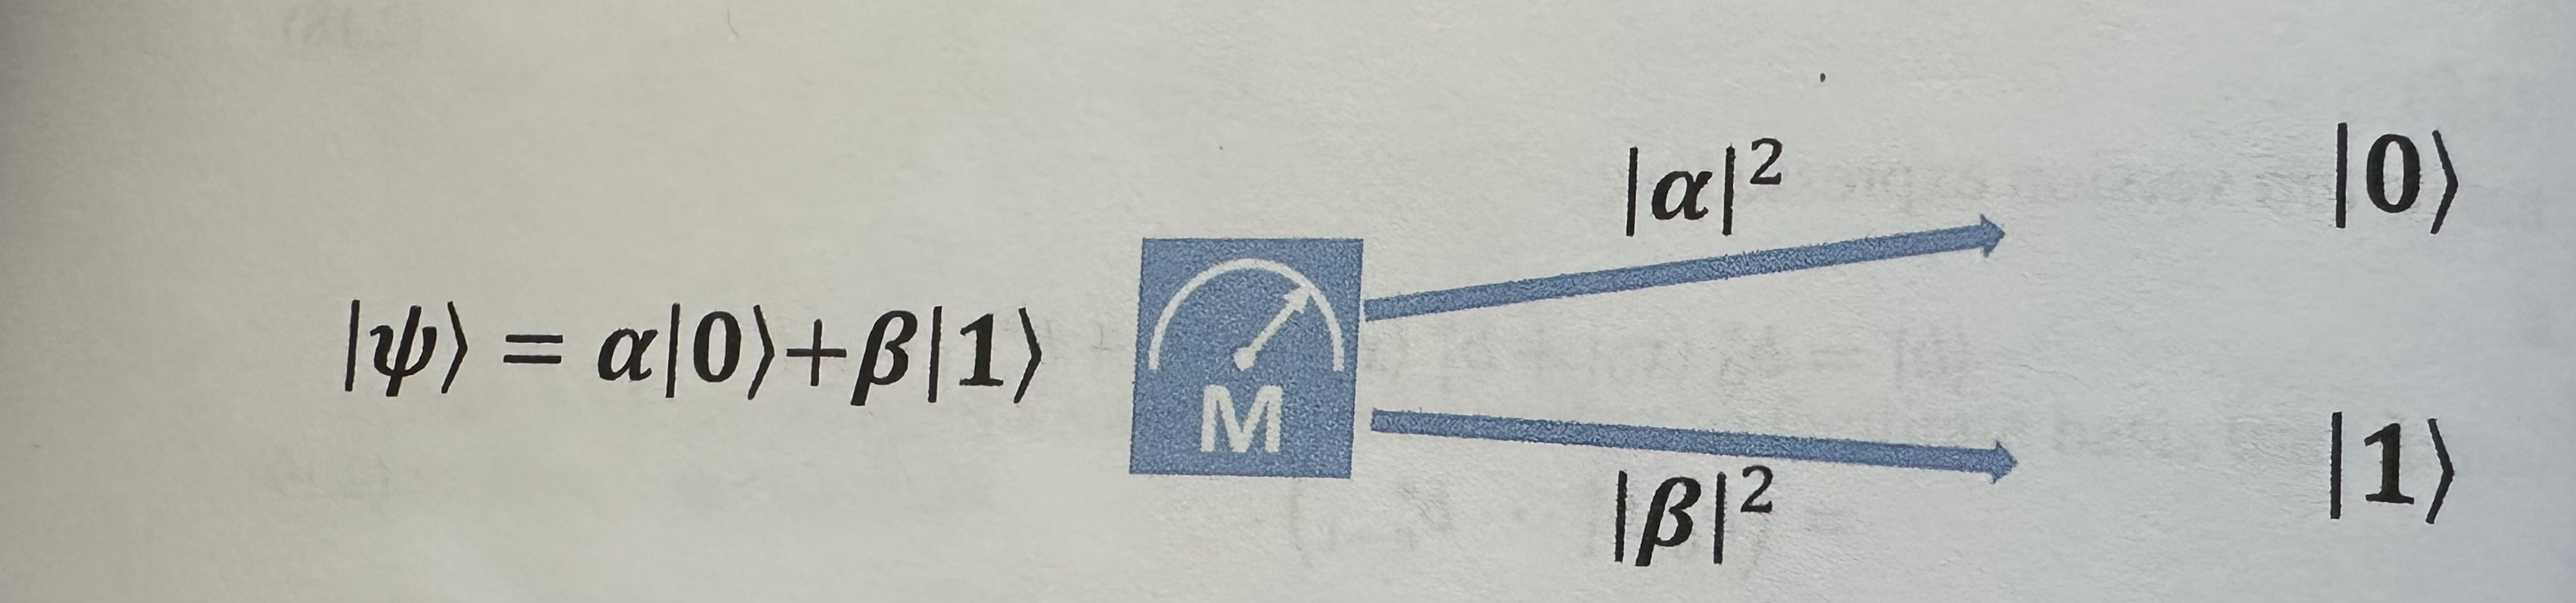
\includegraphics[scale=0.35, angle=0]{Fig.2.3.jpeg}

Fig.2.3 Upon meausrement, a state will collapse to one of the basis states with a probability equal to the square fo the magnitude of the corresponding coefficient

and the probability it will collapse to $\ket{1}$ is

\begin{equation}
 Prob(\ket{1})=\beta\beta^* = |\beta| ^2   \tag{2.22}
\end{equation}

\end{document}